\subsection{Alternative Splicing}

L'alternative splicing è un meccanismo utilizzato dalle cellule per produrre proteine (o per meglio dire, \textit{isoforme proteiche}) diverse dallo stesso gene che viene utilizzato da oltre il 75\% dei geni umani \cite{wang2008alternative}. Diversi studi (come \cite{tazi2009alternative} e \cite{rockenstein1995levels}) dimostrano come l'alternative splicing giochi un ruolo fondamentale nello sviluppo di diverse malattie, come ad esempio il cancro o la sindrome di Alzheimer.

Considerando un generico frammento di DNA, esso può essere diviso in esoni (parti codificanti) e introni (parti non codificanti). Durante la fase di Trascrizione gli introni vengono rimossi e la Timina viene trasformata in Uracile, ottenendo pre-mRNA. A questo punto, in un normale processo di Splicing, tutti gli esoni vengono utilizzati, nell'ordine in cui appaiono nel pre-RNA, per ottenere una proteina.

\begin{figure}[h!]
	\centering
	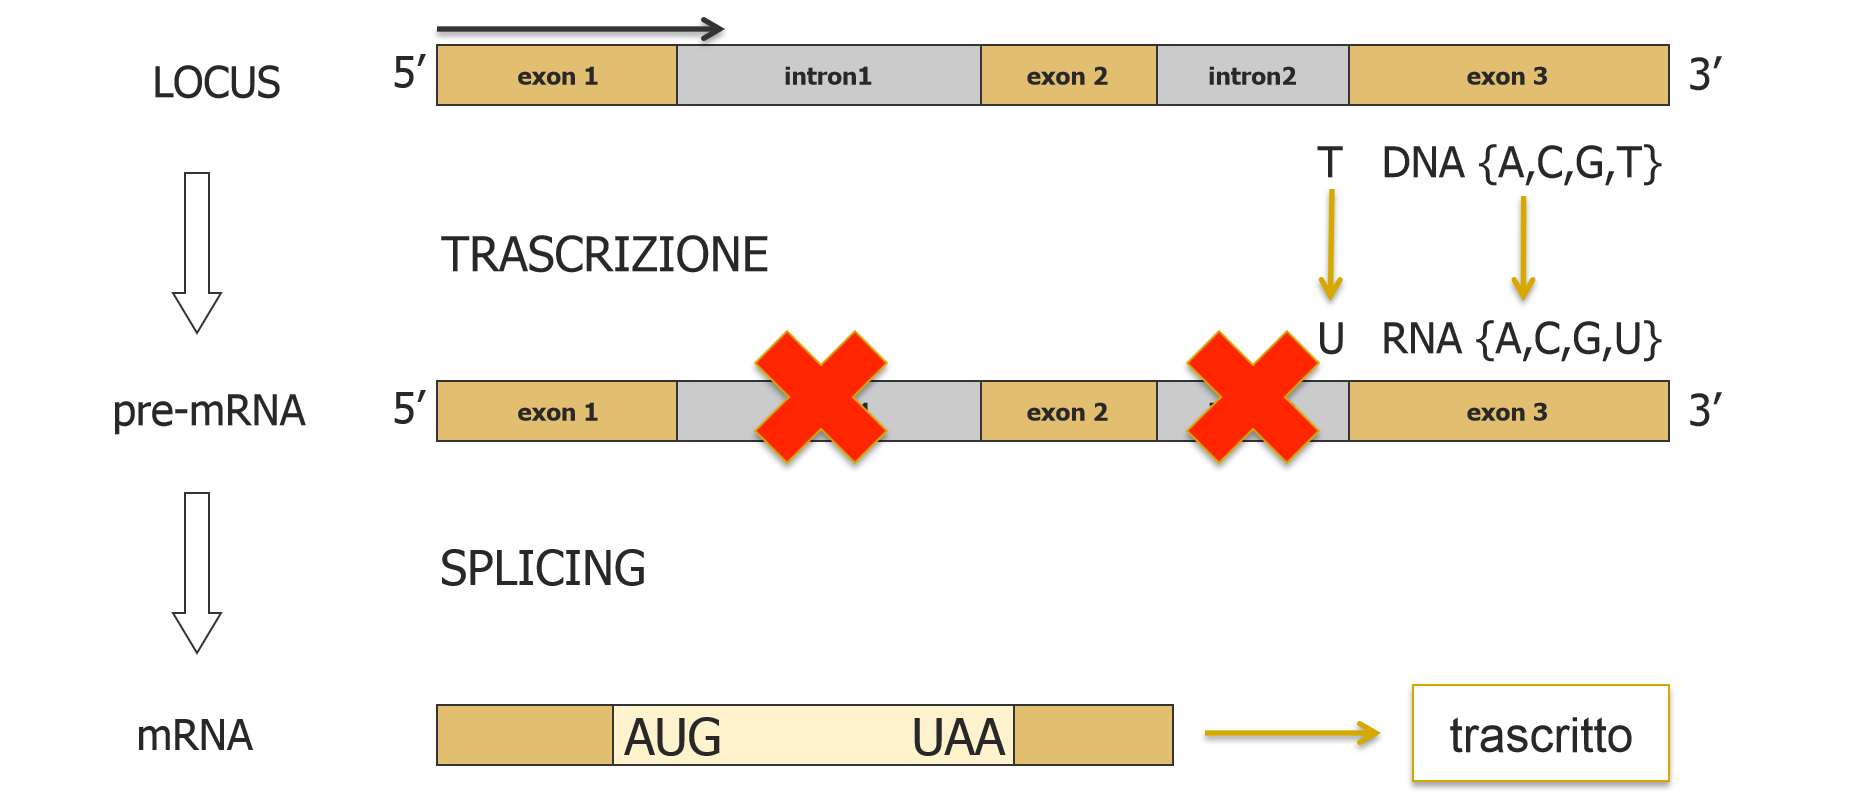
\includegraphics[width=\linewidth]{images/splicing.png}
  \caption{Trascrizione e Splicing}
  \label{fig:Splicing}
\end{figure}

Nel caso di un evento di Alternative Splicing, questo non accade: alcuni esoni potrebbero infatti non essere utilizzati, o apparire in un ordine diverso. Vengono riconosciuti 5 tipi di eventi di Alternative Splicing:

\begin{enumerate}
	\item \textbf{Exon Skipping}: Un esone non appare nel trascritto; quando gli esoni sono più di uno, si parla di \textbf{Multiple Exon Skipping}
	\item \textbf{Mutually Exclusive Exons}: Due esoni non compaiono mai in uno stesso trascritto contemporaneamente
	\item \textbf{Alternative 5' Donor Site}: Parte di un introne nel 5' diventa un esone
	\item \textbf{Alternative 3' Acceptor Site}: Parte di un introne nel 3' diventa un esone
	\item \textbf{Intron Retention}: Parte di un esone diventa un introne
\end{enumerate}

ASGAL è in grado di rilevarli tutti tranne il caso 2.

\newpage

\begin{figure}[t!]
	\centering
	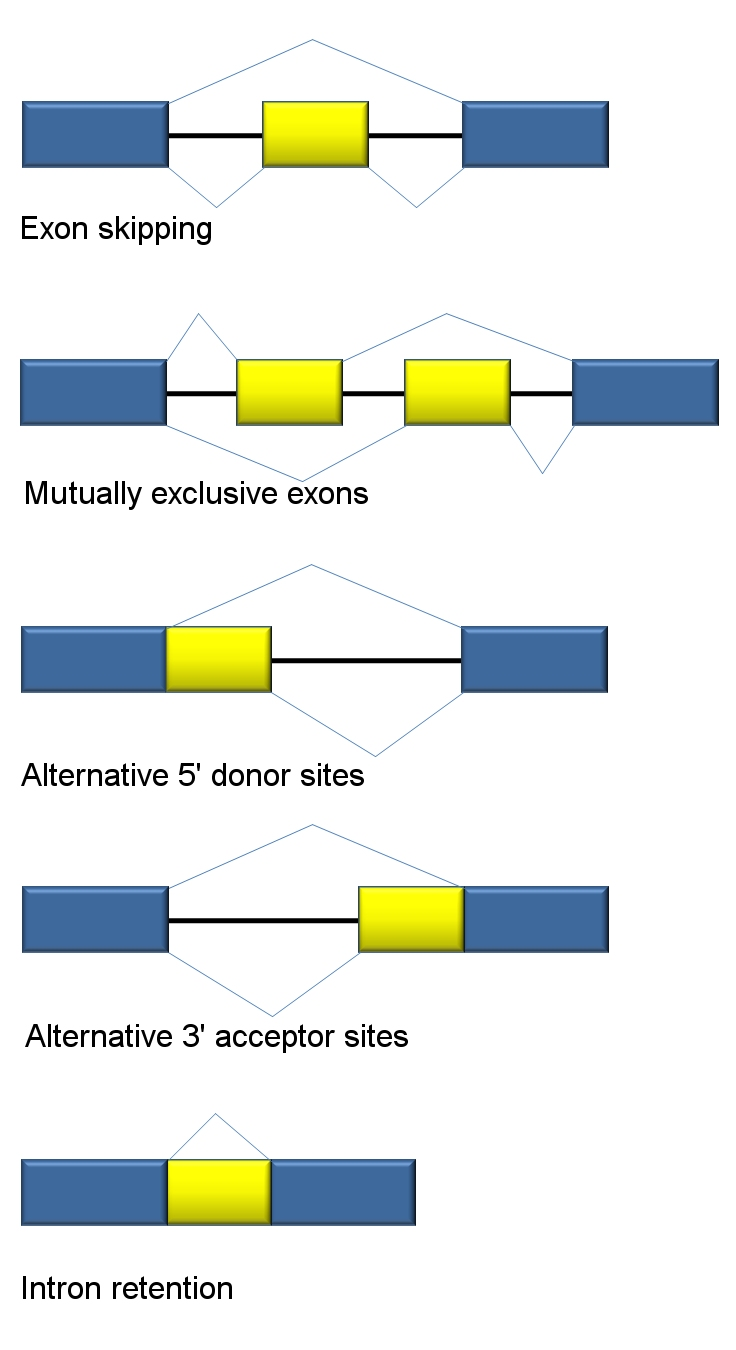
\includegraphics[height=10cm,width=10cm]{images/alternativesplicingevents.jpg}
  \caption{I diversi tipi di Alternative Splicing}
  \label{fig:AlternativeSplicingTypes}
\end{figure}

\subsection{Paired-End Reads}
Le paired-end reads consistono nell'estrazione di due letture da un singolo frammento di DNA, contrariamente alle single-end reads che ne estraggono solo una. Sono prodotte da sistemi NGS, e la loro preparazione è molto semplice: una volta stabilita la grandezza della singola lettura, viene estratta la lettura sull'estremità sinistra, il campione viene girato, e viene estratta nuovamente l'estremità sinistra (ottenendo quindi l'estremità destra); viene generalmente fornita anche la distanza tra le due letture.

\begin{figure}[h!]
	\centering
	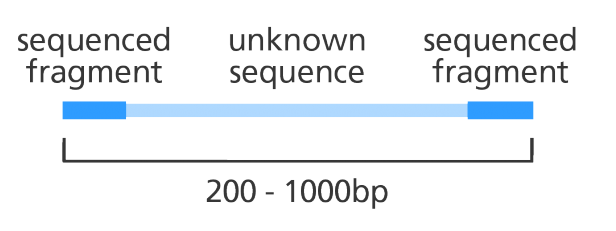
\includegraphics{images/pairedendreads2.png}
  \caption{Read paired-end}
  \label{fig:PairedEndReads}
\end{figure}